\section{Using RKWard - an example RKWard session}
\label{sec:using_RKWard}
This section describes an example RKWard session, in order to give an idea
what working with RKWard is like in practice.
The session is organized along the routine tasks of importing,
analyzing, and visulazing data. In this example, we assume that an experimental
treatment was given to 20 test subjects and the values of the dependent
variable before and after the treatment should be compared. 

\subsection{Importing data}
\label{sec:importing_data}
Data which was saved as or exported to CSV format for example from a
spread sheet application. RKWard's import plugin can
comfortably read it into a new \proglang{R} object.
The import dialog (``File->Import->Import
format->Import Text / CSV data'') assists during the
selection of the data by a common point and click interface (Figure~\ref{fig:import_data}A). Within our
example ``comma'' and ``period'' were chosen via ``Quick mode'' as field
separator character and decimal point character respectively.

The corresponding \proglang{R} code would read as:

\code{read.csv(file=/media/software/experiment.txt, 
na.strings = NA, nrows = -1, skip = 0,
check.names = TRUE, strip.white = FALSE, blank.lines.skip = TRUE)}


Checking the ``Edit Object'' box will automatically open a data editor tab
showing the imported data (Figure~\ref{fig:import_data}B).

\begin{figure}[htp]
 \centering
 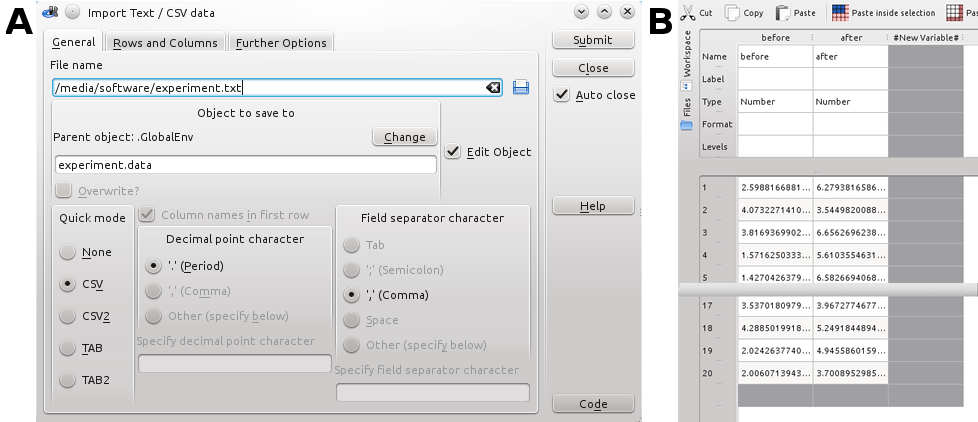
\includegraphics[width=15.5cm]{../figures/import_data.png}
 \caption{A) CSV import dialog. Useful defaults for a variety of common text separated value formats can
  be set using the ``Quick Mode'' selector on the left. Beyond that, many options can be customized. B) Data editor. The imported CSV
  data from experiment.txt are presented (data visually trimmed).}
 \label{fig:import_data}
\end{figure}

\subsection{Conducting a Student's t-test}
\label{sec:conducting_ttest}
To test the hypothesis that the given treatment significantly increased
the values of the dependent variable, a Student's
t-test for a paired sample is applied. In the variable slot on the left
side you select the variables from the unfolded
\proglang{R} object containing the table of imported data (Figure~\ref{fig:t_test}A).

\begin{figure}[htp]
 \centering
 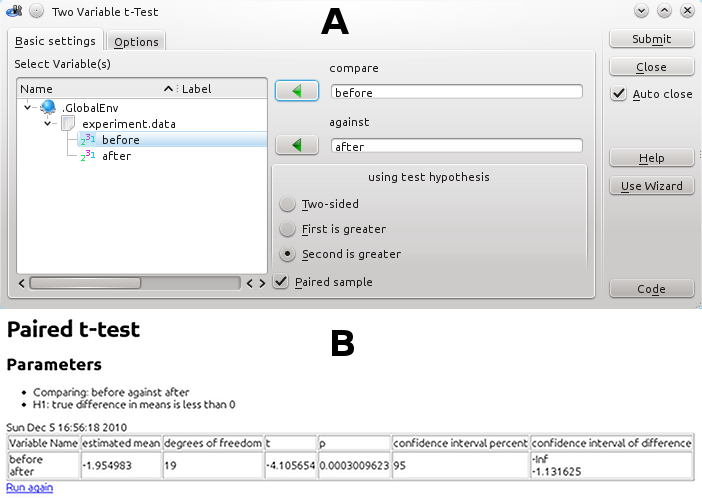
\includegraphics[width=15.5cm]{../figures/t-test.png}
 \caption{A) Student's t-test dialog for a two variables. B) Test results in \proglang{HTML} format.}
 \label{fig:t_test}
\end{figure}

After the ``Submit'' button was pressed, RKWard opens the output document
to show the results (Figure~\ref{fig:t_test}B).

\subsection{Creating a plot}
\label{sec:create_plot}
To visualize the test data, ``Boxplot'' is chosen from the ``Plots'' menu
and variables selected are as for the Student's t-test.
The dialog allows to define custom variable labels (Figure~\ref{fig:boxplot1}).

\begin{figure}[htp]
 \centering
 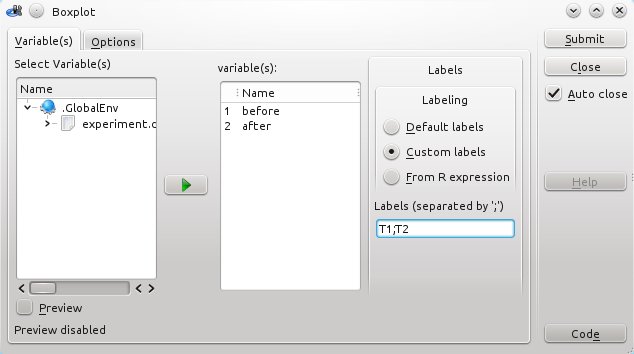
\includegraphics[width=15.5cm]{../figures/boxplot1.png}
 \caption{Boxplot dialog.}
 \label{fig:boxplot1}
\end{figure}

Checking the ``Preview'' box will open a graphics window, show the plot as
it is configured and update the window on changes in real time. From
that window it can be exported directly to several data formats as
well (Figure~\ref{fig:boxplot2}).

\begin{figure}[htp]
 \centering
 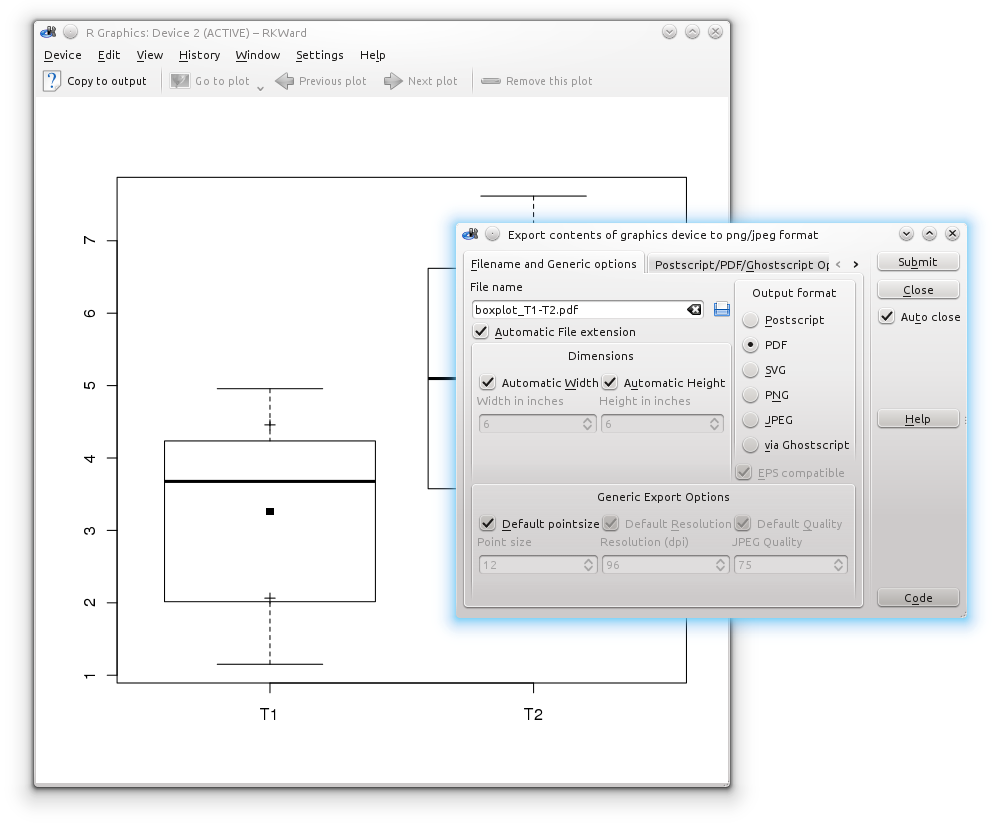
\includegraphics[width=15.5cm]{../figures/boxplot2.png}
 \caption{Plotted data and plot export dialog.}
 \label{fig:boxplot2}
\end{figure}
